\documentclass[10pt,journal,cspaper,compsoc]{IEEEtran}
\usepackage[]{lipsum}
\usepackage{cite}
\usepackage{amsmath,amssymb}
\usepackage{algorithm}
\usepackage{algorithmic}
\usepackage{multirow}
\usepackage{mathtools}

\usepackage[aboveskip=8pt]{caption}

\usepackage[dvips]{graphicx}
\DeclareGraphicsExtensions{.pdf}
\usepackage[american]{babel}

\usepackage{tabularx}


\usepackage{url}
\usepackage{cvpr}
\usepackage{multicol}
\usepackage{stfloats}
\usepackage{fixltx2e}
\usepackage{caption}
\usepackage{microtype}
\usepackage{subcaption}

\usepackage[export]{adjustbox}
\usepackage[bookmarks=false,colorlinks=true,linkcolor=black,citecolor=black,filecolor=black,urlcolor=black]{hyperref}

\newcommand{\cb}[1]{\textbf{#1}}
\newcommand{\ct}[1]{\fontsize{7pt}{1pt}\selectfont{#1}}
\newcommand{\tn}[1]{\footnotesize{#1}}
\newcommand{\code}[1]{\texttt{#1}}
\newcolumntype{x}{>\small c}


\def\cls{\mathit{cls}}
\def\reg{\mathit{reg}}

%\renewcommand{\floatpagefraction}{0.1}
%\renewcommand{\bottomfraction}{0.1}
%\renewcommand{\topfraction}{1}
%\renewcommand{\textfraction}{0.0}
\renewcommand{\dbltopfraction}{1.0}
\renewcommand{\dblfloatpagefraction}{0.0}

\newcommand*{\figuretitle}[1]{%
    {\centering%   
    \textbf{#1}%   
    \par\medskip}% 
}

\newcommand{\tabincell}[2]{\begin{tabular}{@{}#1@{}}#2\end{tabular}}

\DeclarePairedDelimiter\ceil{\lceil}{\rceil}
\DeclarePairedDelimiter\floor{\lfloor}{\rfloor}


\title{Exposure Fusion}

\author{
    \IEEEauthorblockN{Dario Loi}
    \IEEEauthorblockA{(1940849)},
    \IEEEauthorblockN{Flavio Gezzi}
    \IEEEauthorblockA{(1958690)}
}

\IEEEcompsoctitleabstractindextext{%
\begin{abstract}
    Exposure Fusion é una tecnica che permette di trasformare una sequenza di immagini
    con diversi valori di esposizione in un unica immagine ad alto range dinamico (HDR), 
    per questo progetto ci siamo concentrati sull'implementazione originale di questo metodo\cite{stanford:exposure_fusion}, ottenendo buoni risultati in termini qualitativi, 
    abbiamo inoltre implementato una versione alternativa, che fa uso di alcuni step di pre-elaborazione, ottenendo risultati piú
    robusti e ovviando a una serie di limitazioni dovute a i mezzi a nostra disposizione.
\end{abstract}
}

\begin{document}

\maketitle



\section{Introduzione}

Il metodo originale é dettagliato con precisione nel materiale originale\cite{stanford:exposure_fusion},
in questo documento ci limiteremo a riassumere i passaggi principali. 

Per prima cosa, data una sequenza di immagini $ I = \{ I_0, \dots, I_N \} $, si calcolano
tre metriche per ogni immagine $ I_i $, il contrasto, la saturazione e l'esposizione:

\begin{equation}
    \label{eq:contrast}
    C_i = L \circledast G_i
\end{equation}

Dove $ L $ é un filtro di Laplace, $ \circledast $ é la convoluzione e $ G_i $ é l'immagine $ i $-esima in
grayscale.

\begin{equation}
    \label{eq:saturation}
    S_{i\ j,k} = \sum_{u=1}^3 \left( I_{i\ j,k,u} - \frac{1}{3} \sum_{v=1}^3 I_{i\ j,k,v} \right)^2
\end{equation}

\begin{equation}
    \label{eq:exposure}
    E_{i\ j,k} = \prod_{u=1}^3 \left( \exp(-\frac{(I_{i\ j,k,u} - 0.5)^2}{2 \sigma^2}) \right)
\end{equation}

Il valore di $ \sigma $ in (\refeq{eq:exposure}) é stato scelto empiricamente, e 
corrisponde a $\sigma = 0.2$.

Successivamente, si utilizzano queste tre metriche per calcolare una maschera di fusione $W_i$:

\begin{equation}
    \label{eq:fusion_mask}
    W_i = C_i \cdot S_i \cdot E_i
\end{equation}

La maschera di fusione é normalizzata in modo che la somma di tutti i suoi valori sia 1, andando 
cosi a costituire una distribuzione di probabilitá.

\begin{equation}
    \label{eq:fusion_mask_normalization}
    \hat{W}_i = \frac{W_i}{\sum_{j=0}^N W_j}
\end{equation}

Infine, per ottenere l'immagine finale in HDR, si costruiscono due piramidi, una gaussiana 
e una laplaciana, a partire rispettivamente dalle maschere di fusione e dalle immagini 
originali. 
Le piramidi vengono poi fuse, ottenendo una nuova piramide laplaciana, che viene fatta collassare 
in un'immagine finale in HDR.\@

\section{Implementazione}
Abbiamo scelto di fornire un implementazione in Python, disponibile in allegato, che permette di
eseguire sia il metodo originale, sia la versione alternativa. La nostra implementazione
é inoltre provvista di un'interfaccia grafica, che permette all'utente di caricare 
le immagini, di scegliere il metodo da utilizzare e di salvare i risultati.

Per testare l'implementazione abbiamo inoltre fatto riferimento a un implementazione in Python
giá disponibile\cite{github:arpesenti}.

\subsection{Il nostro metodo}

A causa della mancanza di apparecchiature professionali, alcuni dei nostri test sono stati
effettuati su scatti ottenuti da fotocamere mobile, di solito allineati in maniera pessima,
per risolvere questo problema (e per migliorare la qualitá delle immagini) abbiamo inserito 
uno step facoltativo di pre-elaborazione, che permette di allineare le immagini, il metodo 
utilizzato é il seguente:

\begin{enumerate}
    \item Per ogni immagine si applicano le seguenti operazioni:
    \begin{enumerate}
        \item Si equalizza l'istogramma dell immagine, per eliminare eventuali differenze di esposizione
        che porterebbero a falsi positivi.
        \item Si applica un gaussian blur, per eliminare eventuali rumori.
        \item Si converte l'immagine in grayscale.
    \end{enumerate}
    \item Si sceglie l'immagine al centro della sequenza come immagine di riferimento.
    \item Per ogni immagine, si utilizza un feature detector per trovare i punti di interesse, 
    é stato empiricamente scelto di utilizzare ORB\cite{ICCV:ORB}, sebbene ci siano diverse 
    alternative.\cite{Lowe:SIFT, Bay:SURF}
    \item Si costruisce una matrice di omografia tra l'immagine di riferimento e ogni altra immagine, 
    utilizzando i punti di interesse trovati precedentemente, dopo aver opportunamente scartato 
    gli outlier.
    \item Si proiettano le immagini originali (non quelle pre-elaborate) allineandone 
    rispetto all'immagine di riferimento.
\end{enumerate}

Cosi facendo, si ottiene una sequenza di immagini i quali punti di interesse sono allineati,
il metodo é funzionale qualora le immagini siano allineate in modo simile, ma non perfettamente, 
fallisce invece se le deformazioni tra le immagini sono troppo grandi, in questo caso l'oggetto 
di interesse dell'immagine risulta allineato ma si vengono a create degli artefatti in corrispondenza
dei bordi, come si puó vedere nella figura \ref{fig:align_crusader}.

\begin{figure*}[ht]
    \centering
    \figuretitle{Artefatti di allineamento}
    \subfloat[a][Allineata]{
        \includegraphics*[width=0.40\textwidth,height=0.32\textheight]{figures/crusader_ours.png}
    }
    \subfloat[b][Non allineata]{
        \includegraphics*[width=0.40\textwidth,height=0.32\textheight]{figures/crusader_standard.png}
    }
    \caption[Commento.]{Possiamo notare nell'immagine originale (b) gli scatti sono troppo disallineati 
    per permettere la corretta fusione dell'immagine, ció risulta in un immagine finale 
    completamente sfocata, nell'immagine allineata (a) la fusione é effettuata correttamente 
    nelle vicinanze del modellino, in ogni modo, é evidente la presenza di un artefatto di deformazione 
    nell'angolo in alto a sinistra della foto che rende il risultato indesiderabile.}\label{fig:align_crusader}
\end{figure*}

\begin{figure*}[ht]
    \centering
    \figuretitle{Exposure Fusion - Immagini Reflex} 
    \subfloat[Input 1]{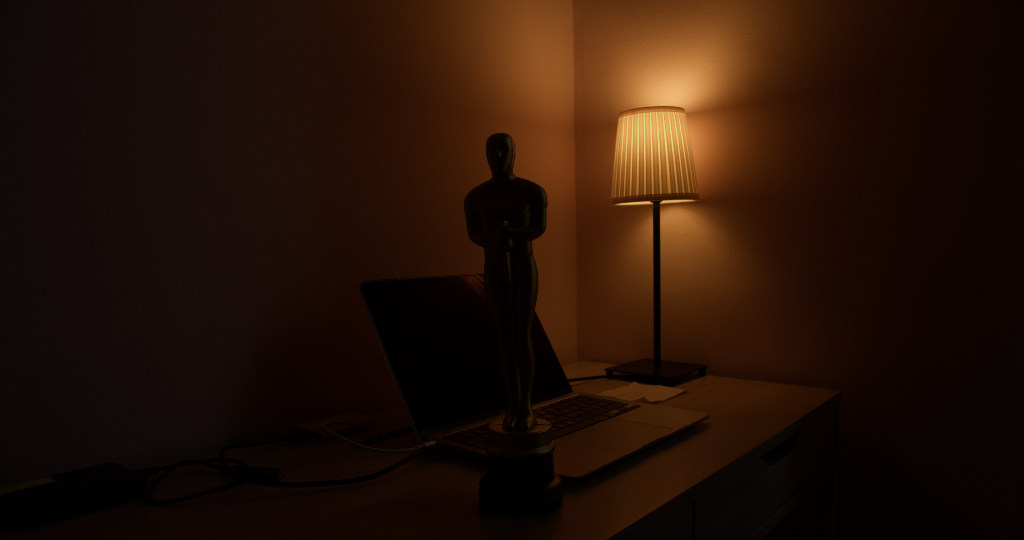
\includegraphics[width=0.33\textwidth,height=0.13\textheight]{figures/test_1.png}} \hfill
    \subfloat[Input 2]{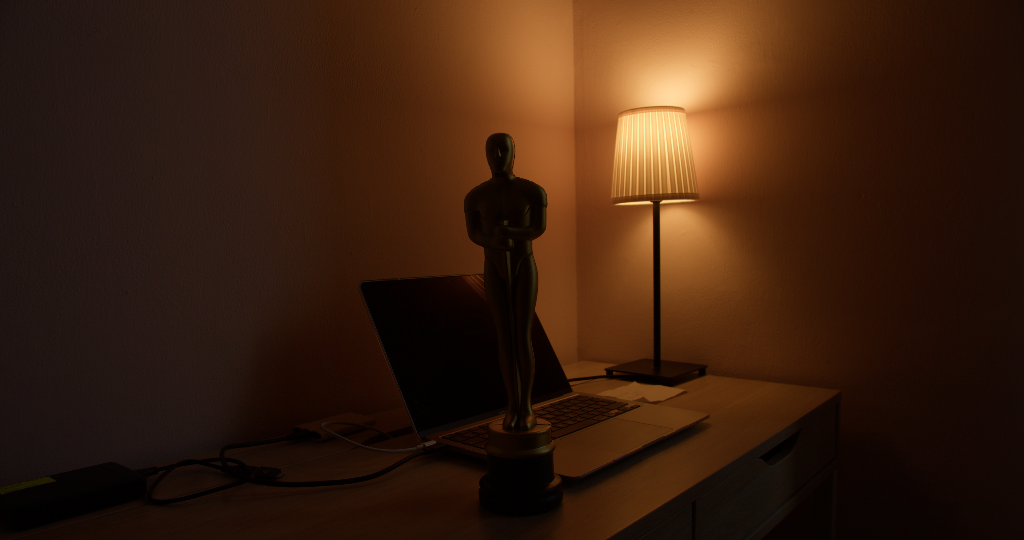
\includegraphics[width=0.33\textwidth,height=0.13\textheight]{figures/test_2.png}} \hfill
    \subfloat[Input 3]{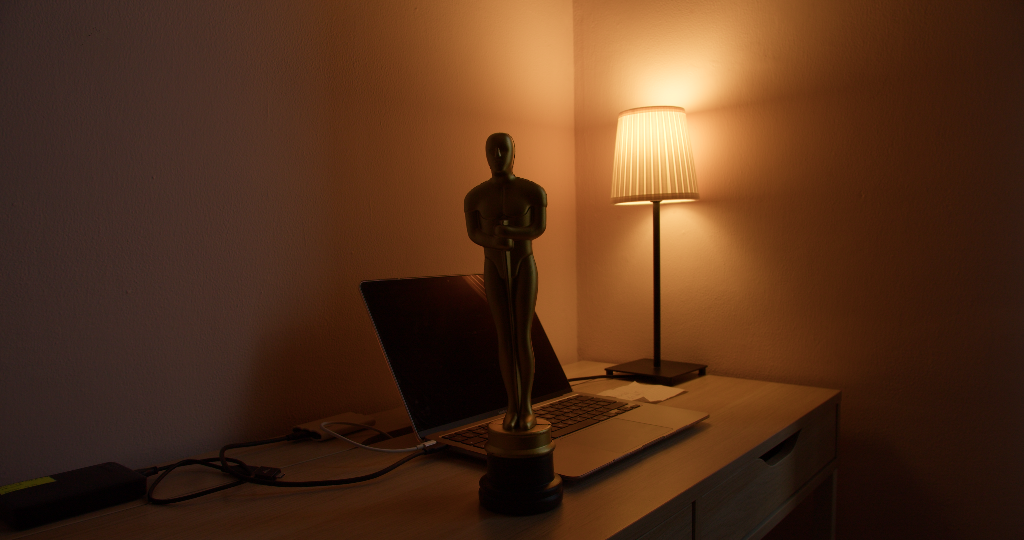
\includegraphics[width=0.34\textwidth,height=0.13\textheight]{figures/test_3.png}}\\[0pt]
    \subfloat[Input 4]{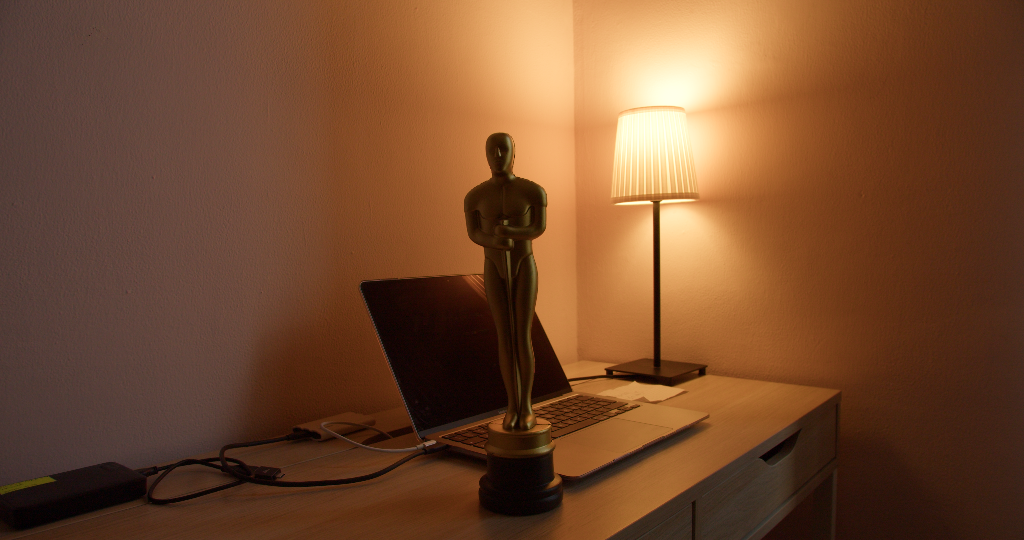
\includegraphics[width=0.33\textwidth,height=0.13\textheight]{figures/test_4.png}} \hfill
    \subfloat[Input 5]{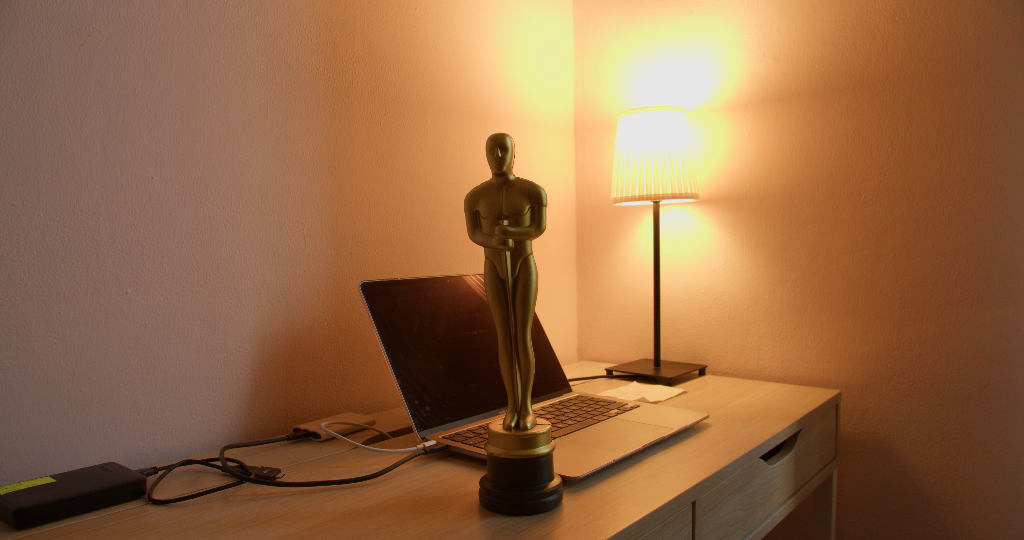
\includegraphics[width=0.33\textwidth,height=0.13\textheight]{figures/test_5.png}} \hfill
    \subfloat[Output HDR]{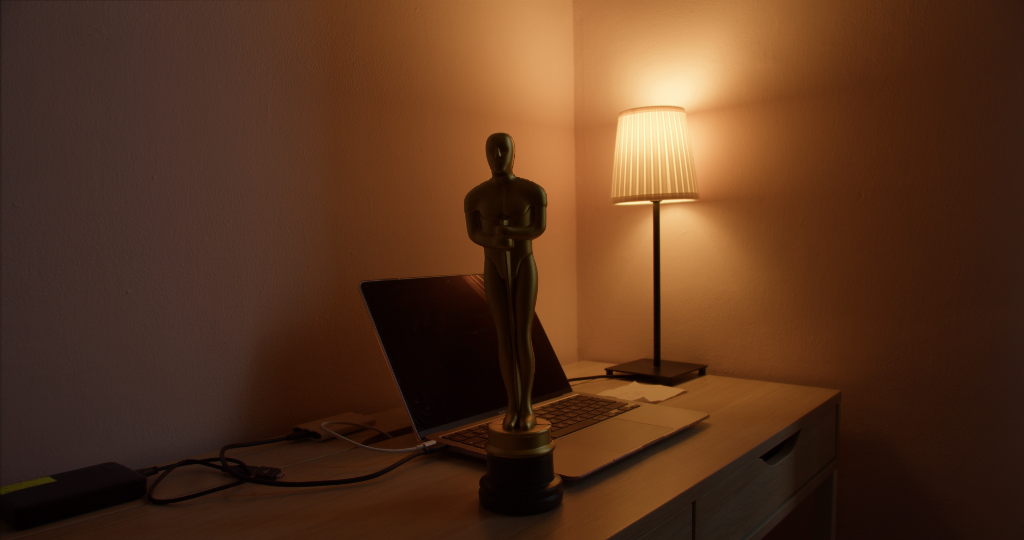
\includegraphics[width=0.34\textwidth,height=0.13\textheight]{figures/out_1.png}} \hfill

    \caption[Commento Reflex.]{
        Abbiamo applicato il nostro metodo ad una serie di immagini (a, b, c, d, e) ottenute con una fotocamera reflex,
        l'immagine finale (f) non dimostra alcun tipo di deformazione da allineamento, L'illuminazione della lampada 
        é molto piú dolce rispetto alle immagini con forte esposizione, mentre sulla statuetta sono visibili un buon 
        numero di dettagli. Possiamo inoltre notare che, in modo analogo a quanto visto per le immagini con flash nella 
        paper originale\cite{stanford:exposure_fusion}, le immagini LDR ad alta esposizione sono fortemente illuminate 
        dalla lampada, l'immagine HDR riesce a ridistribuire l'illuminazione in modo tale da consentire una maggior 
        chiarezza delle aree in penombra.}\label{fig:fusion}

\end{figure*}

\begin{figure*}[ht]
    \centering
    \figuretitle{Exposure Fusion - Ulteriori Esempi Reflex} 
    \subfloat[Input 1]{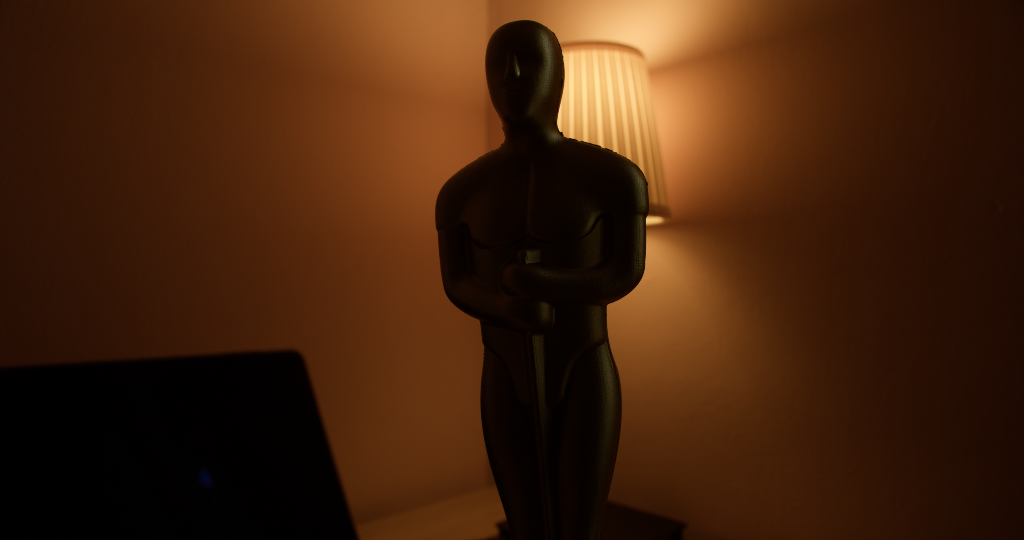
\includegraphics[width=0.33\textwidth,height=0.13\textheight]{figures/test_2_1.png}} \hfill
    \subfloat[Input 2]{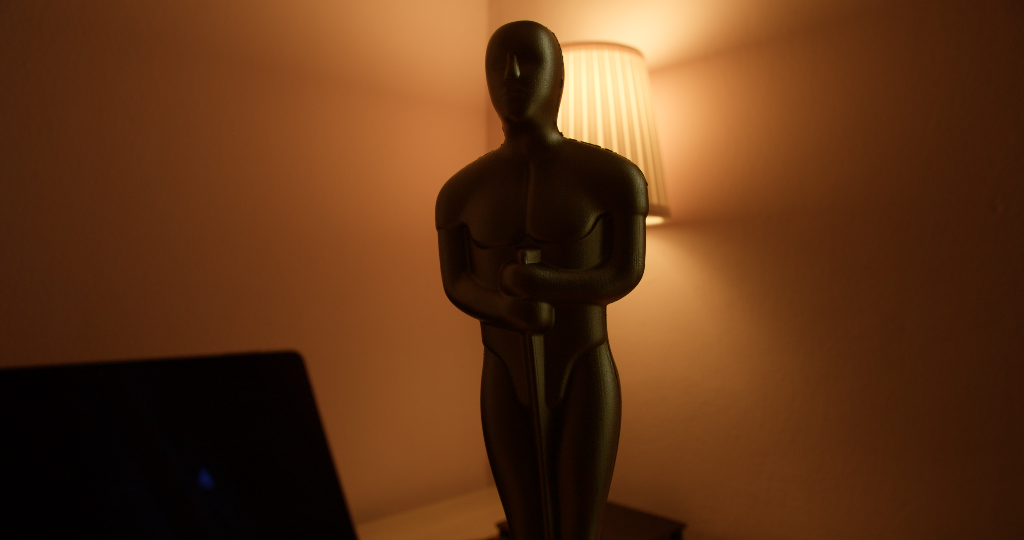
\includegraphics[width=0.33\textwidth,height=0.13\textheight]{figures/test_2_2.png}} \hfill
    \subfloat[Input 3]{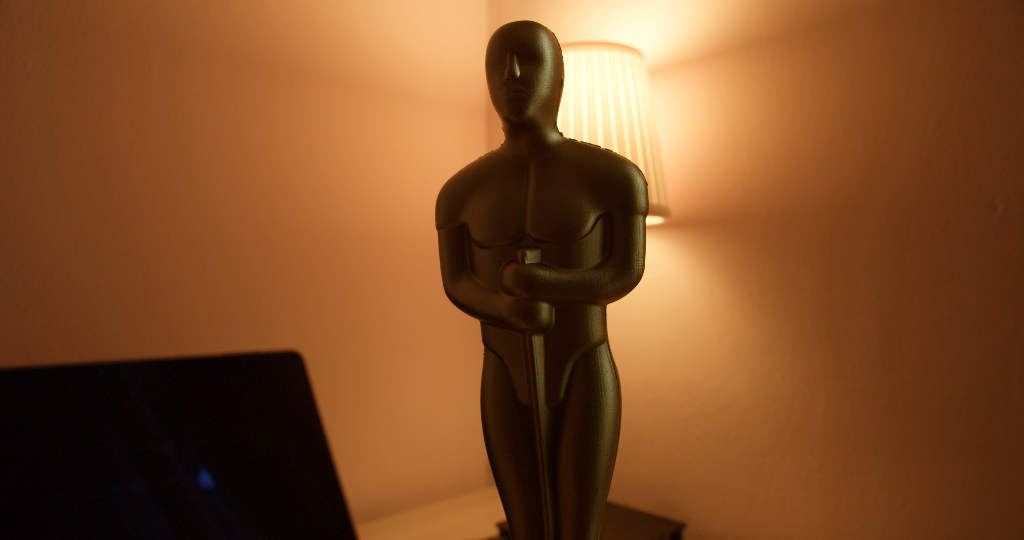
\includegraphics[width=0.34\textwidth,height=0.13\textheight]{figures/test_2_3.png}}\\[0pt]
    \subfloat[Input 4]{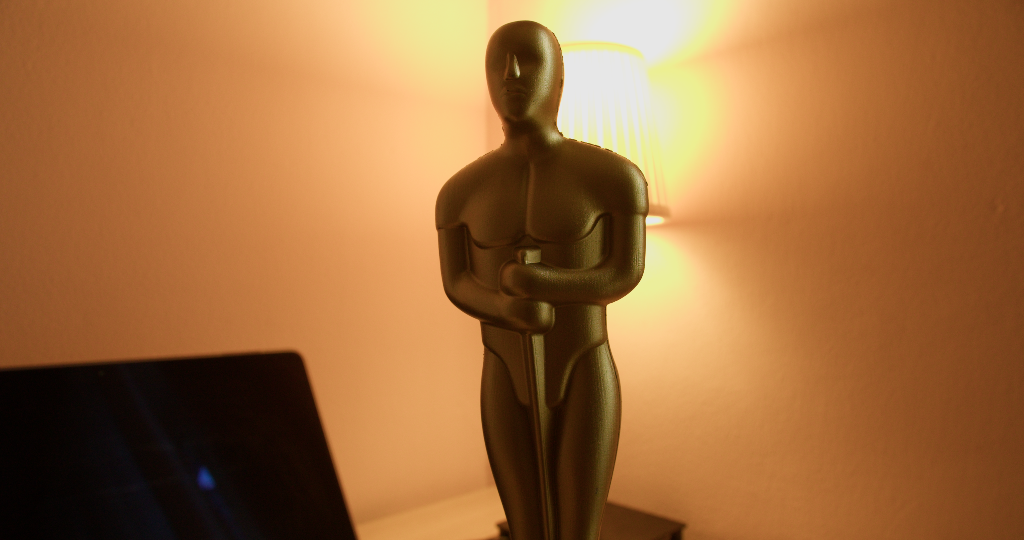
\includegraphics[width=0.33\textwidth,height=0.13\textheight]{figures/test_2_4.png}} \hfill
    \subfloat[Input 5]{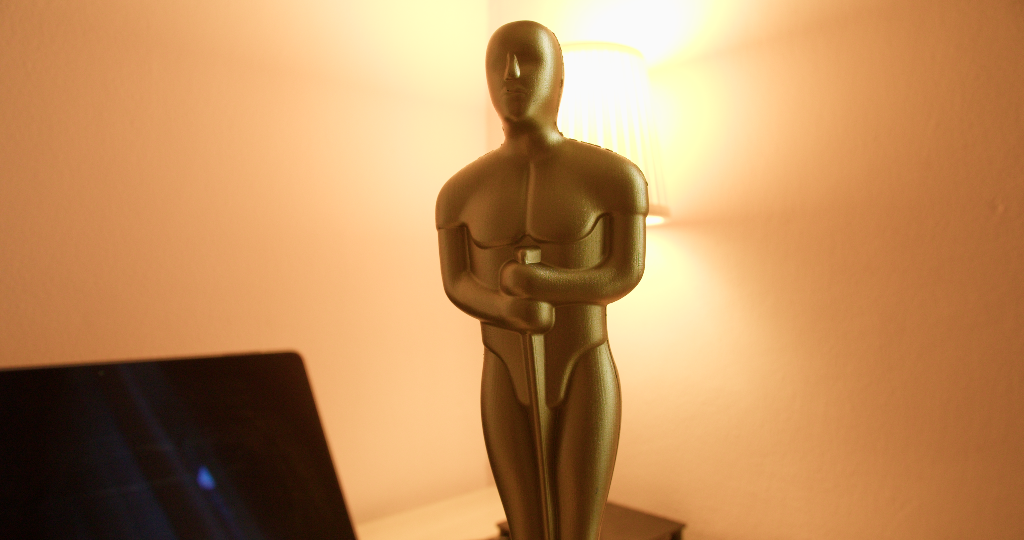
\includegraphics[width=0.33\textwidth,height=0.13\textheight]{figures/test_2_5.png}} \hfill
    \subfloat[Output HDR]{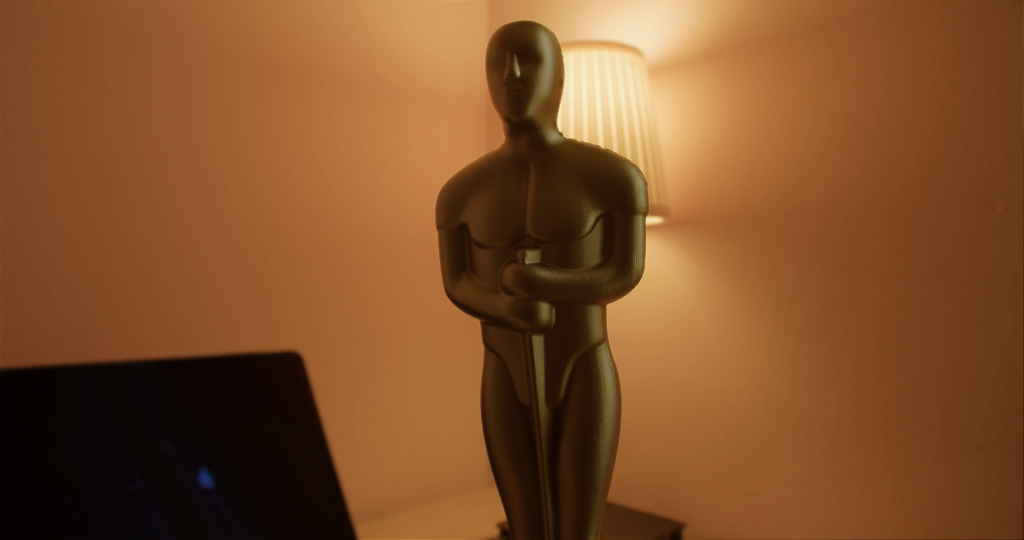
\includegraphics[width=0.34\textwidth,height=0.13\textheight]{figures/out_2.png}} \hfill

    \caption[Commento Reflex.]{
        In seguito possiamo osservare un altra applicazione del nostro metodo, anche qui abbiamo una sequenza di immagini 
        (a, b, c, d, e) ottenute con una fotocamera reflex, l'immagine finale (f) non dimostra alcun tipo di deformazione
        e, analogamente al caso precedente.
        }\label{fig:fusion}

\end{figure*}


\section{Risultati}

Il nostro metodo é stato testato su una serie di immagini ottenute con una fotocamera mobile, insieme 
a un numero limitato di immagini ottenute con una fotocamera reflex. 

In seguito, verranno mostrati e commentati diversi risultati ottenuti con il nostro metodo, le immagini 
verranno rese disponibili in allegato in modo da rendere possibile la riproducibilitá dei risultati.

Generalmente, il nostro metodo é in grado di ottenere risultati simili a quelli della paper originale, 
presentando allo stesso tempo le stesse limitazioni.

É infatti noto agli autori originali che il metodo 
presenta degli artefatti a bassa frequenza quando la profondita delle piramidi Gaussiane e Laplaciane é troppo 
bassa, questo problema é risolvibile aumentando la profonditá, cio peró aumenta il tempo di computazione e 
puó risultare in un secondo tipo di artefatto, in cui i valori di intensitá non sono piú presenti nell'intervallo $(0, 1]$, 
questo problema é risolto da metodi piú recenti\cite{hessel:exp_fusion}, ma rimane nella nostra implentazione.

\section{Conclusioni}

Crediamo di aver raggiunto risultati solidi, sviluppando un modulo che permette di implementare Exposure Fusion 
cosi come descrita originariamente. 

Questo documento é accompagnato dalle seguenti risorse:

\begin{itemize}
    \item Il codice sorgente del modulo, importabile come classe in qualsiasi file python.
    \item Un file Jupyter Notebook contenente esempi di utilizzo del modulo, atti a riprodurre 
    i risultati mostrati in questo documento.
    \item Un applicazione GUI realizzata con la libreria python TKinter, che permette l'interazione     
    con exposure fusion attraverso un interfaccia grafica.
\end{itemize}

\bibliographystyle{IEEEtran}
\bibliography{ref}

\end{document}